\documentclass[11pt]{article}
% CREATED BY  © ALI MOHAMED, 2017 

%PACKAGES

\usepackage[Swedish]{babel}
\usepackage[T1]{fontenc}
\usepackage[utf8]{inputenc}
\usepackage{graphicx}
\usepackage{fancyhdr}
\usepackage{pdflscape}
\usepackage{amsmath}
\usepackage{listings}

\renewcommand\listfigurename{}
%


%PACKAGE-SETTINGS

\usepackage%[margin=2.5cm,a4paper]
{geometry}
		  
\usepackage[colorlinks, citecolor=black,
   		 	filecolor=black, linkcolor=black,
    		urlcolor=blue]{hyperref}
%

% RENEWING BASIC LENGTHS

\setlength{\parindent}{0em}
\setlength{\parskip}{0mm}



% CONFIGURATION-FANCYHDR (HEADER & FOOTER)
\renewcommand{\headrulewidth}{0pt}
\renewcommand{\footrulewidth}{0.5pt}
\pagestyle{fancy}
\fancyhf{}
\rfoot{\thepage(7)}
\rhead{}

	\fancypagestyle{plain}{			% REDEFINING PAGESTYLE PLAIN		
		\fancyhf{}
		\renewcommand{\headrulewidth}{0pt} 		
		\fancyfoot[RO]{\thepage}
	}
%
\usepackage{tikz}
\usetikzlibrary{shapes,arrows}
\begin{document}
\newcommand{\no}{1}
\newcommand{\subject}{Positions- och varvtalsreglering av hjulen}

\newgeometry{margin=2.5cm}

\thispagestyle{empty}
\parbox[h!][\textheight][t]{\textwidth}{
\parbox[h!][\textheight][t]{0.19\textwidth}{

\vspace*{0.075\textheight}
\hspace*{0.15\textwidth}
\rule[\textheight]{1.5pt}{0.85\textheight}
}
\parbox[h!][0.85\textheight][t]{0.76\textwidth}{
\vspace{10em}

{\huge Inlämning \no} \\[0.1cm]
{\Large{ERE103, Reglerteknik D3}} \\[0.8cm]
{\Large \bf \subject} \\ [1cm]
{\Large Ali Mohamed, almoha@student.chalmers.se\\[0.3em]
Ali Mohamud, almoh@student.chalmers.se
\\[0.8cm]
15 November, 2017}
 \\[0.39\textheight]
Avdelningen för Elektroteknik. Institutionen för System och reglerteknik\\
Chalmers tekniska högskola
}}
\restoregeometry
\tableofcontents
\pagestyle{empty}
\newpage
\setcounter{page}{1}
\pagestyle{fancy}
\section{Laplacetransformeringar och överföringsfunktioner}
Systemet består av en elektrisk och mekanisk komponent, nämligen DC- motorn med tillhörande hjul. Effekten som motorn genererar regleras med spänningen $u$, som ger upphov till en ström $i_a$. Strömmen kommer att således ge upphov till ett vridmoment $\tau$, vridmomentet är direkt proportionerligt emot strömmen med en proportionalitetskonstant.
\\[2em]

Genom att härleda ekvationen $F=ma$ och nyttja sambandet att $a(t) = \frac{\partial}{\partial t}v(t) = \frac{\partial^2}{\partial t^2}s(t)$ återfinns en förta ordningens differentialekvation som beskriver det mekaniska sambandet.
\begin{equation}
I\dfrac{\partial}{\partial t}\omega(t) = \tau_d(t)-b\cdot\omega(t); \quad I = I_m +I_h
\end{equation}
Genom att tillämpa Kirchoffs spänningslag d.v.s att $\sum\limits_{i=1}^{n} u_i = 0$ fås nedanstående samband.
\begin{equation}
R_ai_a(t)+L_a\dfrac{\partial}{\partial t}i_a(t) + u_m(t) = u(t)
\end{equation}
Eftersom att systemet innehåller en induktor bildas ett mot-EMK\footnote{Motriktad elektromotorisk kraft} som är proportionerlig emot DC-motorns vinkelhastighet $\omega$. Relationen ges av
\begin{equation}
u_m(t) = K_u\omega(t)
\end{equation}
På samma sätt är strömmen $i_a$ proportionerlig emot DC-motorns vridmoment $\tau$. Relationen ges av
\begin{equation}
\tau_d(t) = K_mi_a(t)
\end{equation}
\subsection{Identifiera överföringsfunktionen: Elektrisk}
Identifiera, med hjälp av modellen för DC-motorn, $G_e(s)$ i följande uttryck.
$$\tau_d(t) = G_e(s)(U(s)-K_u\Omega(s))$$ \\[0.5em]
\textbf{Lösning}
\begin{equation*}
\begin{split}
G_e(s)&= \dfrac{\tau_d(t)}{U(s)-K_u\Omega(s)} =\dfrac{K_mI_a(s)}{U(s)-K_u\Omega(s)} = \dfrac{K_mI_a(s)}{R_aI_a(s)-L_asI_a(s)+U_m(s)-K_u\Omega(s)}\\
&=\dfrac{K_mI_a(s)}{I_a(s)(R_a+L_as)+U_m(s)-K_u\Omega(s)}= \dfrac{K_mI_a(s)}{I_a(s)(R_a+L_as)+K_u\Omega(s)-K_u\Omega(s)}\\
&=\dfrac{K_m}{R_a+L_as}
\end{split}
\end{equation*}
\newpage
\subsection{Identifiera överföringsfunktionen: Mekanisk}
Identifiera, med hjälp av modellen för hjulet, $G_m(s)$ i följande uttryck.
$$\Omega(s)=G_m(s)\tau_d(s); \quad
\text{där} \ \ \mathcal{L}\{\omega(t)\}=\Omega(s)$$
Bearbetning av ekvation (1) ger följande samband
\begin{equation*}
\begin{split}
&=I\dfrac{\partial}{\partial t}\omega(t) = \tau_d(t)-b\cdot\omega(t) \Rightarrow
I\dfrac{\partial}{\partial t}\omega(t) +b\cdot\omega(t) = \tau_d(t) \Rightarrow \omega(t)(\dfrac{\partial}{\partial t}I+b) = \tau_d(t)\\
\omega(t)&= \dfrac{\tau_d(t)}{\dfrac{\partial}{\partial t}I+b} = \underbrace{\tau_d(t)}_{\mathcal{L}^-1\{\tau_d(s)\}}\cdot\underbrace{(\dfrac{\partial}{\partial t}I+b)^-1}_{\mathcal{L}^-1\{G_m(s)\}}\\
G_m(s)&=(Is+b)^{-1} = \dfrac{1}{Is+b}
\end{split}
\end{equation*}

\subsection{Bestäm tidskonstanten för det mekaniska och elektriska systemen}
Överföringsfunktionen $H(s)$ är ett bråk som kan omskrivas som $\frac{P(s)}{Q(s)}$, där dessa är täljar- och nämnarpolynom. Rötterna till $P(s)$ betecknas som nollställen medan rötterna till $Q(s)$ betecknas som poler. Om polerna är imaginära kommer systemet att oscillera, storleken på oscillationen beror på storleken av imaginärdelen. \\[0.5em]
Parametern T i $Q(s)=sT+1$ är ett mått på systemets tempo och benämns för tidskonstant. Tidskonstanten är tid det tar för stegstvaret att uppgå till $63\%$ av slutsvärdet. I tidsdomänen blir ${\mathcal{L}}^-1\{Q(s)\} = K_0e^{-t/T}$.\\[1em]
$
\begin{cases}
G_m(s)= \dfrac{1}{Is+b}, \quad {\mathcal{L}}^-1\{G_m(s)\} = e^{-b/I}    \\[1em]
G_e(s)= \dfrac{K_m}{L_as+R_a}, {\mathcal{L}}^-1\{G_e(s)\} = K_me^{-R_a/L_a}\\
\end{cases}
$\\[0.5em]
Genom att ansätta variabler $b,I,R_a,L_a$ finner man att det elektriska systemet är snabbare.

\subsection{Bestäm överföringsfunktionen}
Bestäm överföringsfunktionen från spänningen u till hjulets varvtal $\omega$, d.v.s.
$$
G_{u\omega}=\dfrac{\Omega(s)}{U(s)}
$$
Genom att substituera $i_a(t)$ mot ekv.(4) fås uttrycket
\begin{equation*}
u(t)=R_a\dfrac{\tau_d(t)}{K_m}+L_a\dfrac{\partial}{\partial t}\cdot\Big( \dfrac{\tau_d}{K_m}\Big)+K_u\omega(t) = \dfrac{\tau_d(t)}{K_m}\Big(R_a+L_a\dfrac{\partial}{\partial t}\Big)+k_u\omega(t)
\end{equation*}
\begin{equation*}
\mathcal{L}\{u(t)\} =U(s)= \dfrac{\tau_d(s)}{K_m}\Big(R_a+L_as\Big)+K_u\Omega(s)
\end{equation*}\newpage
Vidare är $G_m(s)=\dfrac{1}{Is+b}$ vilket medför att hjulets vinkelhastighet $\mathcal{L}\{\omega(t)\}$ är
\begin{equation*}
\Omega(s)=\dfrac{\tau_d(s)}{Is+b}
\end{equation*}
Genom att ansätta de härledda uttrycken för $\Omega(s)$ och $U(s)$ i överföringsfunktionen $G_{uw}$ blir överföringsfunktionen
\begin{equation*}
\begin{split}
G_{uw} &= \dfrac{\dfrac{\tau_d(s)}{Is+b}}{\dfrac{\tau_d(s)}{K_m}\Big(R_a+L_as\Big)+K_u\Omega(s)} = \dfrac{\dfrac{\tau_d(s)}{Is+b}}{\dfrac{\tau_d(s)}{K_m}\Big(R_a+L_as\Big)+K_u\dfrac{\tau_d(s)}{Is+b}}\\
&=\dfrac{K_m}{K_mK_u+(R_a+L_as)(Is+b)}
\end{split}
\end{equation*}
\section{Varvtalsreglering}
\subsection{Blockschema för systemet}
\tikzstyle{block} = [draw, rectangle, 
    minimum height=3em, minimum width=3em]
\tikzstyle{sum} = [draw, circle, node distance=3cm]


\tikzstyle{input} = [coordinate]
\tikzstyle{output} = [coordinate]
\tikzstyle{pinstyle} = [pin edge={to-,thin,black}]
\newcommand{\summa}{\huge$\sum_{}^{}$}

% The block diagram code is probably more verbose than necessary
\begin{tikzpicture}[auto, node distance=2cm,>=latex']
    % We start by placing the blocks
    \node [input, name=input] {};
    
    \node [sum, right of=input, ] (summa) {\summa};
    \node [block, right of=summa, ] (F) {F(s)};
    \node [sum, right of=F] (sum2) {\summa};
    \node [block, right of=sum2, ] (G) {$G_e(s)$};
    
    \node [block, above of=sum2] (K) {$K_u$};       
    \node [block, right of=G] (G2) {$G_m (s)$};
    \node [sum, below of= sum2] (omega) {$\Omega$} ;
    
    \draw [->] (summa) -- node {E} (F);
    \draw [->] (F) -- node[pos=0.95] {$ + $} node [near end] [name=u] {u} (sum2);
    \draw [->] (sum2) -- node[name=gc] {} (G);
    \draw [->] (K) -- node [pos=0.95] {$ - $} node [near end][name=ksys] {} (sum2);
    \draw [->] (G) -- node[name=gc] {T} (G2);
    \node [output, right of=G2] (output) {out};
   
    \draw [->] (input) -- node[pos=0.95] {$ + $} node [near end] [name=line] {$\Omega_r$} (summa);
     
    
    \draw [->] (G2) -- node [name=y] {$\Omega$}(output);
    \draw [->] (y) |- node  {}(K);
    \draw [-] (y) |- node  {}(omega);
    \draw [->]	(omega) -| node[pos=0.95] {$-$} node [near end]   {}(summa);
    
    

\end{tikzpicture}
\subsection{Bestäm det kvarstående felet}
Det kvarstående felet beräknas genom att beräkna gränsvärden för reglerfelet $e_s$ d.v.s $\lim_{t \to \infty} e_s(t)$. Genom att laplacetransformera reglerfelet och tillämpa slutvädersstaten blir gränsvärdet $\lim_{s \to 0}sE(s)$. Nedan tillkommer lite ekvationer och samband som finns i labb-PM:et. 

\begin{equation}
F(s)=\dfrac{U(s)}{E(s)} \Rightarrow U(s) = F(s)E(s)
\end{equation}
\begin{equation}
w_r(t)=w_o\sigma(t) \Rightarrow \Omega_r(s)=w_o\dfrac{1}{s}, \quad \sigma(t) \ \text{är ett enhetssteg}
\end{equation}
\begin{equation}
G_{uw} = \dfrac{\Omega_r(s)}{U(s)} \Rightarrow \Omega(s) = G_{uw}U(s) \Rightarrow \Omega(s) =G_{uw}F(s)E(s)
\end{equation}
\begin{equation}
U(s)=F(s)\overbrace{(\Omega_r(s)-\Omega(s))}^{E(s)}
\end{equation}\\[1em]
\begin{equation*}
\begin{split}
E(s)&= \Omega_r(s)-\Omega(s)=\Omega_r(s)-G{uw}U(s) = \Omega_r(s)-G_{uw}F(s)E(s)\\
&=\Omega_r(s)(1+F(s)G_{uw}(s))^{-1} = \dfrac{\Omega_r(s)}{1+F(s)G_{uw}(s)} \\ &=\dfrac{\dfrac{\omega_o}{s}}{1+F(s)\dfrac{K_m}{K_mK_u+(R_a+L_as)(b+Is)}}
\end{split}
\end{equation*}
\subsubsection{P-reglering}
\begin{equation*}
\begin{split}
\lim_{s \to 0}sE(s)&=\lim_{s \to 0}  \dfrac{\omega_0}{1+\dfrac{K_mK_p}{K_mK_u+(R_a+L_as)(b+Is)}} = \dfrac{\omega_0}{1+\dfrac{K_mK_p}{K_mK_u+R_ab}}\\[0.5em]
&=\dfrac{w_0(K_mK_u+R_ab)}{K_mKp+K_mK_u+R_ab}
\end{split}
\end{equation*} 
\subsubsection{PI-reglering}
\begin{equation*}
\begin{split}
&=\lim_{s \to 0}sE(s) = \lim_{s \to 0}  \dfrac{\omega_0}{1+\frac{K_ps+K_i}{s}\dfrac{K_m}{K_mK_u+(R_a+L_as)(b+Is)}}\\ &= \lim_{s \to 0}  \dfrac{\omega_0s}{1+\frac{K_ps+K_i}{s}\dfrac{K_m}{K_mK_u+(R_a+L_as)(b+Is)}} = \lim_{s \to 0} \dfrac{\omega_0s}{s+\dfrac{K_m(K_ps+K_i)}{K_mK_u+(R_a+L_as)(b+Is)}} \\
&=\dfrac{0}{\dfrac{K_mK_i}{K_mK_u+R_ab}} = 0
\end{split}
\end{equation*}
\subsection{Jämför P-,I- och PI-reglering}
$
F(s)=
\begin{cases}
K_p, \quad \quad \quad \quad \ \ 
 \text{P-reglering} \\[0.5em]
\dfrac{K_ps+K_i}{s} \quad \quad \text{PI-reglering}
\end{cases}
$
$L(s)=F(s)G_{uw}(s)\Rightarrow G(s)=\dfrac{L(s)}{1+L(s)}$\\[0.5em]
Värden på de regulatorer som skall jämföras\\[1em]
\begin{tabular}{|l|l|l|}
\hline
Regulatorer&$K_p$&$K_i$ \\ \hline \hline
P&0.5&0 \\ \hline
I&0&4.0 \\ \hline
PI&0.1&4.0 \\ \hline
\end{tabular}
\begin{figure}[h!]
\centering
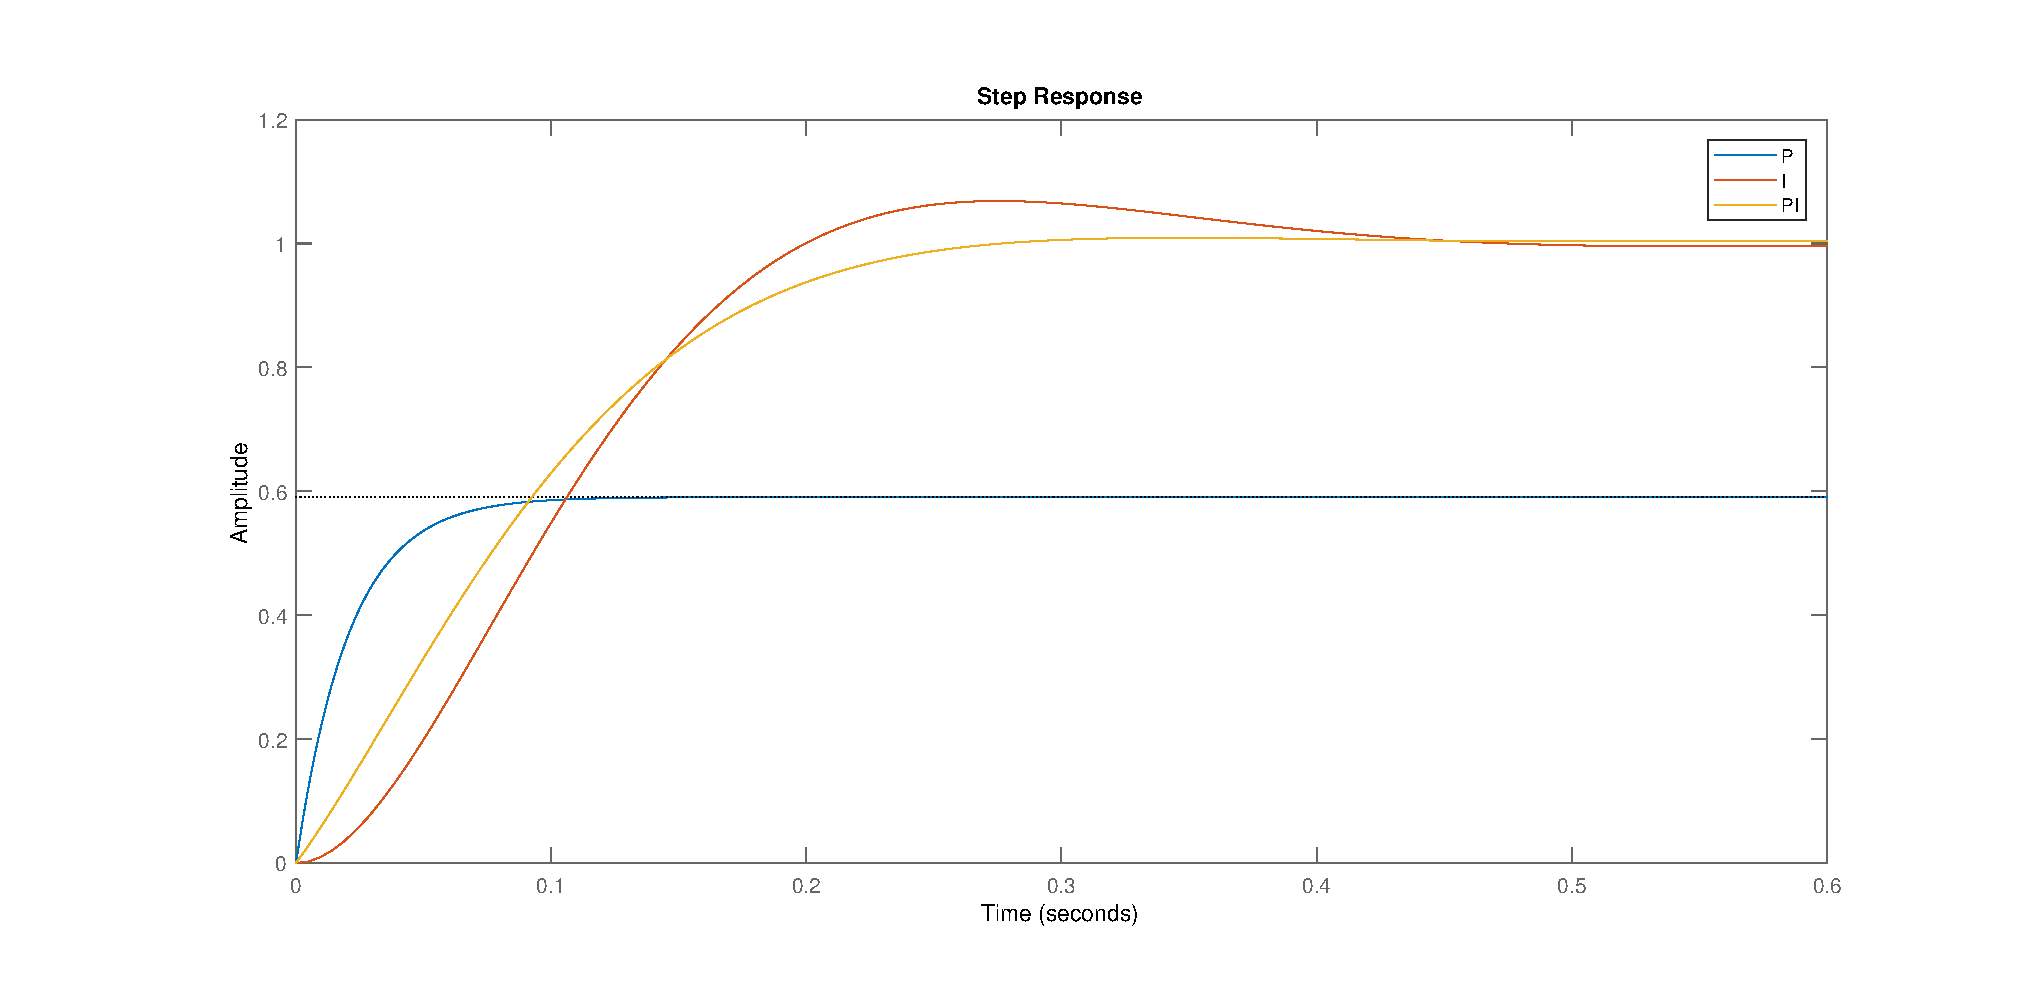
\includegraphics[scale=0.45]{Figures/plot1}
\caption{Mathlab-plot av P-, I- och PI-reglering}
\end{figure}
\section{Positionsreglering}
\subsection{Blockschema för systemet}
\tikzstyle{block} = [draw, rectangle, 
    minimum height=3em, minimum width=3em]
\tikzstyle{sum} = [draw, circle, node distance=3cm]


\tikzstyle{input} = [coordinate]
\tikzstyle{output} = [coordinate]
\tikzstyle{pinstyle} = [pin edge={to-,thin,black}]
\renewcommand{\summa}{\huge$\sum_{}^{}$}

% The block diagram code is probably more verbose than necessary
\begin{tikzpicture}[auto, node distance=2cm,>=latex']
    % We start by placing the blocks
    \node [input, name=input] {};
    
    \node [sum, right of=input, ] (summa) {\summa};
    \node [block, right of=summa, ] (F) {F(s)};
    \node [sum, right of=F] (sum2) {\summa};
    \node [block, right of=sum2, ] (G) {$G_e(s)$};
    
    \node [block, above of=sum2] (K) {$K_u$};       
    \node [block, right of=G] (G2) {$G_m (s)$};
    \node [sum, below of= sum2] (omega) {$\Omega$} ;
    \node [block, right of = G2] (integ){$ 1 /s$};
    
    \draw [->] (summa) -- node {E} (F);
    \draw [->] (F) -- node[pos=0.95] {$ + $} node [near end] [name=u] {u} (sum2);
    
    \draw [->] (sum2) -- node[name=gc] {} (G);
    \draw [->] (K) -- node [pos=0.95] {$ - $} node [near end][name=ksys] {} (sum2);
    \draw [->] (G) -- node[name=gc] {T} (G2);
    \node [output, right of=integ] (output) {out};
   
    \draw [->] (input) -- node[pos=0.95] {$ + $} node [near end] [name=line] {$\phi_r$} (summa);
     
    
    \draw [->] (G2) -- node [name=y] {$\Omega$}(integ);
   \draw [->] (y) |- node  {}(K);
    \draw [->] (integ) -- node [name=outl] {$\phi$}(output);
   \draw [-] (outl) |- node  {}(omega);
    \draw [->]	(omega) -| node[pos=0.95] {$-$} node [near end]   {}(summa);
    
    

\end{tikzpicture}
\subsection{Bestäm kvarstående felet}
Det kvarstående felet bestäms genom att tillämpa slutvädersstaten. Förutsatt att $E(\infty)$ existerar medför detta $\lim_{t \to \infty}e_s(t) = \lim_{s \to 0}sE(s)$ Nedan kommer ekvationer och samband från labb-PM:et.

\begin{equation}
U(s) = F(s)(\Phi_r(s)-\Phi(s))
\end{equation}
\begin{equation}
U(s) = F(s)E(s)
\end{equation}
\begin{equation}
\varphi_r(t)= \varphi_0\cdot\sigma(t) \Rightarrow
\Phi_r(t)=\varphi_0\cdot\dfrac{1}{s}
\end{equation} 
\begin{equation}
\mathcal{L}\{\varphi\}=\mathcal{L}\{\smallint\omega \} = G_{uw}(s)F(s)E(s)\dfrac{1}{s}
\end{equation}\\[1em]
\begin{equation*}
\begin{split}
E(s)&=\Phi_r(s)-\Phi(s)=\Phi_r(s)-G_{uw}(s)E(s)F(s)\dfrac{1}{s} = \dfrac{\Phi_r(s)}{1+G_{uw}(s)F(s)\frac{1}{s}}\\
&=\dfrac{\dfrac{\varphi_0}{s}}{1+\dfrac{F(s)}{s}\dfrac{K_m}{K_mK_u+(R_a+L_as)(b+Is)}} = \dfrac{\varphi_0}{s+F(s)\dfrac{K_m}{K_mK_u+(R_a+L_as)(b+Is)}}
\end{split}
\end{equation*}
\subsubsection{P-reglering}
\begin{equation*}
\begin{split}
\lim_{s \to 0}sE(s) =\lim_{s \to 0} \dfrac{\varphi_0\cdot s}{s+F(s)\dfrac{K_m}{K_mK_u+(R_a+L_as)(b+Is)}} = \dfrac{0}{\cdots} = 0
\end{split}
\end{equation*}
\subsection{Bestäm dämpningsfaktorn och svängningsfrekvensen}
Överfunktionen $G(s)$ lyder
\begin{equation}
G(s) = \dfrac{K\omega_n^2}{s^2+2\zeta\omega_ns+\omega_n^s}
\end{equation}
där $\zeta$ är systemets dämpningsfaktor och $\omega_n$ är systemets naturliga frekvens alt. svängningsfrekvensen. Vidare är systemets  kretsöverföring
\begin{equation}
L(s)=F(s)G_{uw}(s)
\end{equation}
Överföringsfunktionen $G(s)$ bli då 
\begin{equation}
G(s)=\dfrac{L(s)}{1+L(s)} = \dfrac{F(s)G_{uw}(s)}{1+F(s)G_{uw}(s)}
\end{equation}
Från ekvationer (12),(8) finner man
\begin{equation}
\Phi(s) = F(s)G_{uw}(s)(\Omega_r(s)-\Omega(s))\frac{1}{s}
\end{equation}
Genom att multiplicera referenssignalen, börvärdet, $\Omega_r(s)$ med överföringsfunktionen måste utsignalen fås, detta medför att
\begin{equation}
\Omega(s)=G(s)\cdot \Omega_r(s)
\end{equation}
Genom att utveckla ekv.(16)(17) fås
\begin{equation*}
\begin{split}
G(s)&= \dfrac{K_pG_{uw}(s)}{s+K_pG_{uw}(s)} = \dfrac{\dfrac{K_mK_P}{K_mK_u+(R_a+L_as)(b+Is)}}{s+\dfrac{K_mK_p}{K_mK_u+(R_a+L_as)(b+Is)}}\\
&=
\dfrac{K_pK_m}{s(K_mK_p+(R_a)(b+Is))+K_pK_m} =
\dfrac{K_pK_m}{s^2R_aI+R_abs+sK_uK_m+K_pK_m}\\ &=
\dfrac{K_pK_m}{s^2R_aI+s(R_ab+K_uK_m)+K_mK_p} =
\dfrac{\dfrac{K_mK_p}{R_aI}}{s^2+\dfrac{s}{R_aI}(R_ab+K_uK_m)+\dfrac{K_mK_p}{R_aI}}\\
\omega_n&=\sqrt{\dfrac{K_mK_p}{R_aI}}, \quad
\zeta=\dfrac{\dfrac{R_ab+K_uK_m}{R_aI}}{2\omega_n} =\dfrac{R_ab+K_uK_m}{2\sqrt{K_pK_mR_aI}}
\end{split}
\end{equation*}
\subsection{Undersök dämpningen}
\begin{tabular}{|l|l|}
\hline
$K_p$&$\zeta$ \hspace*{1em} \\ \hline \hline 
26.9720 & 0.25 \\ \hline
6.7430&0.5\\ \hline
1.6858&1.0\\ \hline
\end{tabular}
\begin{figure}[h!]
\centering
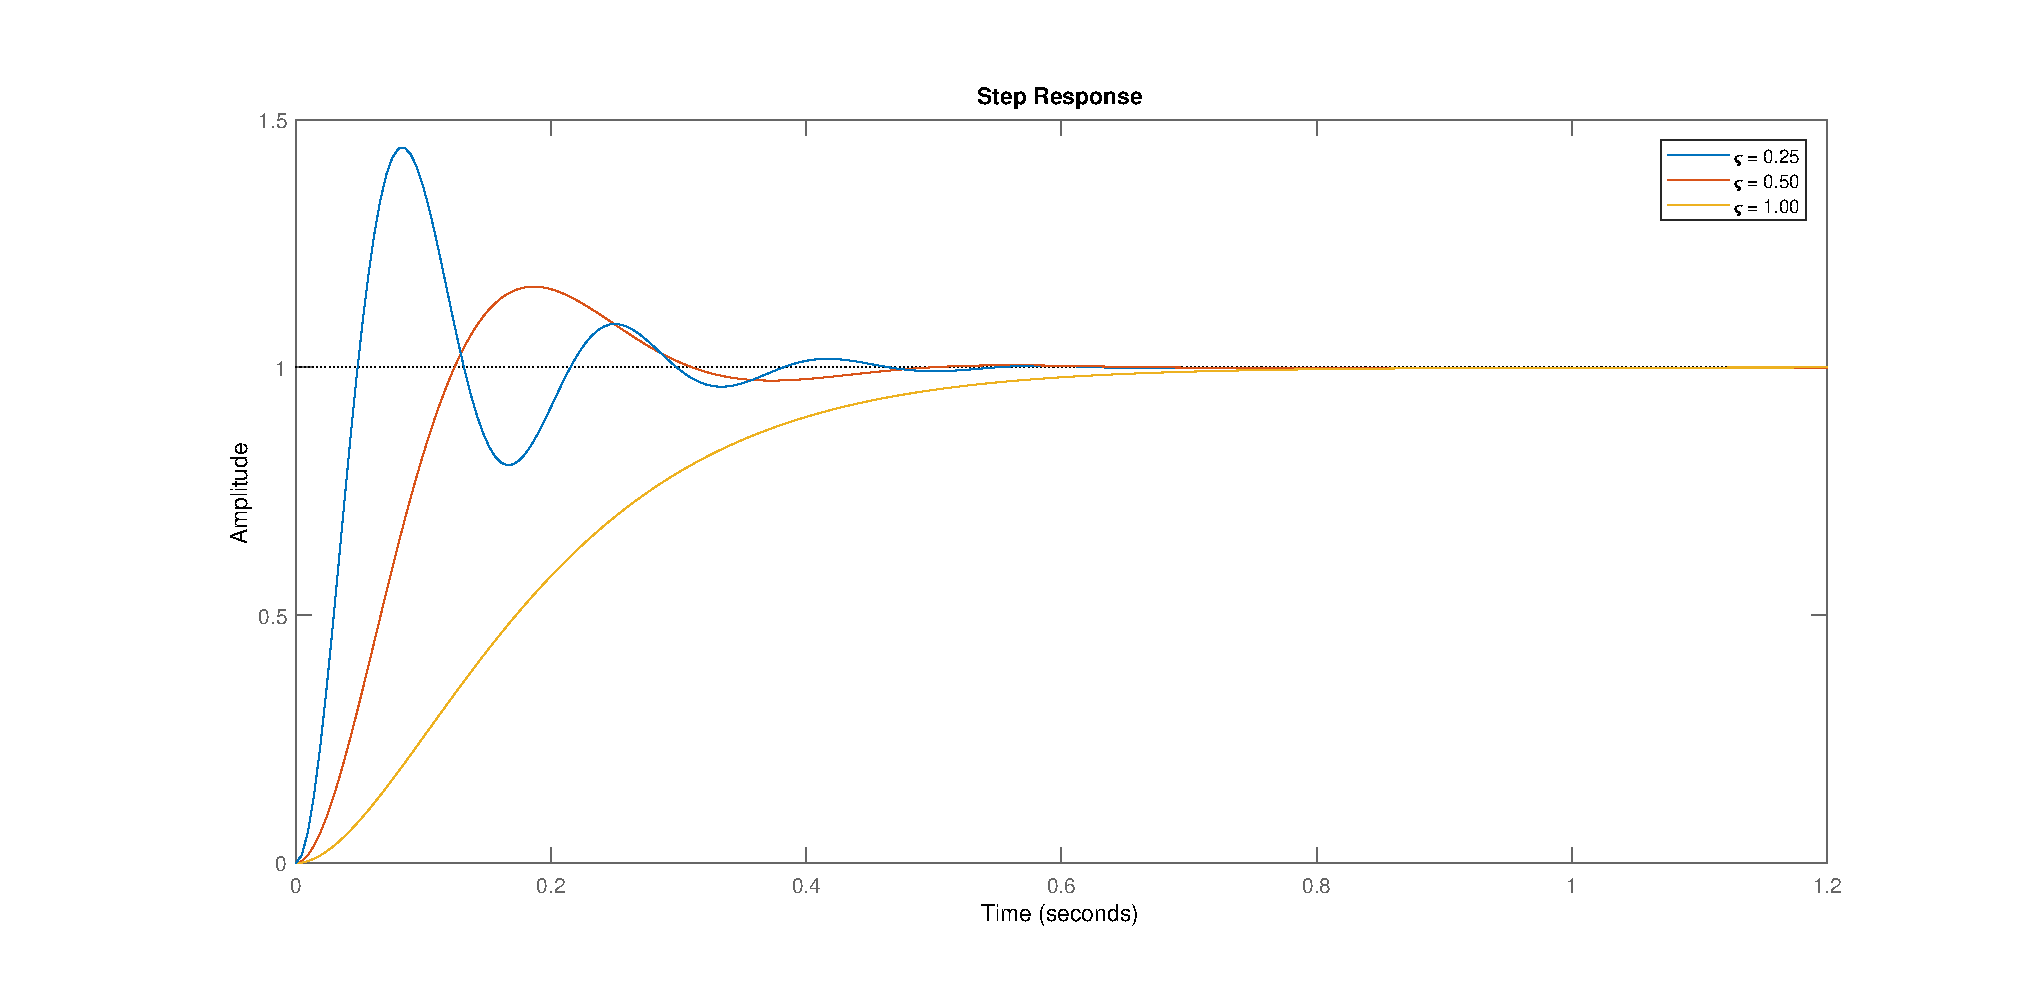
\includegraphics[scale=0.45]{Figures/plot2}
\caption{Matlab-plot av olika dämpningar $\zeta$}
\end{figure}\\[1em]
Vid högre värden på dämpningsfaktorn $\zeta$ till mindre översäng. Vidare tar det längre tid för system med hög dämpningsfaktor att nå sitt slutvärde.

\section{Styrsignal}
Identifiera konstanterna \texttt{C0} och \texttt{C1}. Regulatorn har realiserats till källkoden nedan skriven i språket C. Referensvärdet (börvärdet) ges av \texttt{reference} medan utsignalen (ärvärdet) ges av \texttt{actual\_output}.

\begin{lstlisting}[frame=single]
void loop()
{
h = time_since_last_sample(); // samplingstid
reference = setpoint_generator_pulse(); // Borvarde
double actual_output = getRotSpeed(h); // Arvarde
double e = reference - actual_output; // Reglerfel
P = c0 * e; // P-del
double u = P + I; // Berakna styrsignal
I = I + c1*e; // Uppdatera I-delen
// Begransa styrsignalen -12 <= u <= 12
double saturated_u = constrain(u, -12.0, 12.0);
actuateControlSignal(saturated_u); // Aktuera styrsignal
\end{lstlisting} \vspace*{1em}

\texttt{C0} identifieras som $K_p$ och \texttt{C1} till $K_ih$



\end{document}